\documentclass[10pt, a4paper]{article}

\usepackage[polish]{babel}
\usepackage[T1]{fontenc}
\usepackage[utf8]{inputenc}
\usepackage{float}
\usepackage{graphicx}
\renewcommand{\figurename}{Rysunek}
\renewcommand{\tablename}{Tabell}
\begin{document}
\begin{titlepage}
\begin{center}
\large
\textbf{Mateusz Małowiecki}

\vspace{0.4cm}
\Large
\textbf{Opracowanie noty 4.10 (\textit{Example: The publish-subscribe pattern}) z rozdziału 4 (\textit{Communication}) książki \textit{Distributed Systems}\footnote{Van Steen M., Tanenbaum A.S.: \textit{ Distributed Systems 3rd edition.}}}

\vspace{0.4cm}
\large
\textbf{10 kwietnia 2021}
\end{center}
\end{titlepage}
\section*{Wstęp}
Wzorzec \textit{publikuj-subskrybuj} (ang. \textit{publish-subscribe pattern}) polega na tym, że klient subskrybuje pewne określone komunikaty publikowane przez serwer. W wyniku tego przekazywane są tylko te komunikaty, które są subskrybowane przez klienta, a komunikaty, których nikt nie subskrybuje, będą utracone. Wzorzec ten omówimy za pomocą prostego przykładu.
\section*{Kod serwera}
Na rysunku \ref{fig:mesh1} widzimy przykład naiwnego serwera czasu, który publikuje klientowi swój aktualny czas przez gniazdo \textit{PUB}. Czas jest publikowany co 5 sekund do każdego zainteresowanego klienta.
\begin{figure}[H]
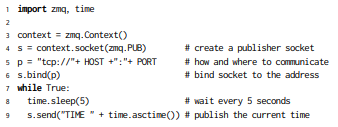
\includegraphics{ps_server}
\caption{Przykładowy kod serwera wzorca \textit{publikuj-subskrybuj}}
\label{fig:mesh1}
\end{figure}
\section*{Kod klienta}
Kod klienta jest w tym przypadku równie prosty, jak kod serwera, co możemy zaobserwować na rysunku \ref{fig:mesh2}. Na początku tworzymy gniazdo \textit{SUB}, które będzie połączone z odpowiednim gniazdem \textit{PUB} serwera. Następnie klient ustawia sobie subskrypcję komunikatów, które mają \textit{TIME} jako swój tag, celem zyskania możliwości odebrania odpowiednich komunikatów. Na koniec klient odbiera pierwsze 5 komunikatów od serwera i drukuje je na standardowym wyjściu. Oczywiście jest to tylko przykład klienta subskrybującego ten serwer. Serwer ten może bowiem mieć wielu różnych subskrybentów i wysyłać komunikaty do każdego z nich.
\begin{figure}[H]
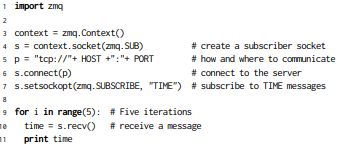
\includegraphics{ps_client}
\caption{Przykładowy kod klienta wzorca \textit{publikuj-subskrybuj}}
\label{fig:mesh2}
\end{figure}
\end{document}